\section{Scikit-learn Modelling}
\label{subsection:scikit-learn}

The Natural Language Toolkit produced some promising models and was quite easy to use. It did not, however, offer much choice or scope for different lines of investigation during model development. Although additional functionality is made available to the developer through a wrapper for Scikit-Learn \cite{scikit-learn}, in this section the NLTK is left behind and focus, instead, turns to the use of Scikit-Learn. Initially, some simple models are quickly developed and explored before attention is given to the more advanced fine tuning operations that are available.

\subsection{Model Development}
Whilst the development of the Scikit-Learn model follows a very similar flow to that utilised for the NLTK model, Scikit-Learn could be considered as a much more advanced toolkit where built-in methods provide a lot of the required data manipulation functionality. As well as this data manipulation functionality Scikit-Learn also provides a better selection of learner algorithms. For the initial investigation, a Naive Bayes and a Support Vertor Machine learner were considered.

The first step in the process is to access the data. Whilst the data could have been accessed directly from the NLTK corpora location, it was decided to pre-process the dataset such that each corpus was consolidated into a single comma separated file with two attributes. The first attribute was the class where \verb|0| was used to represent a bullying sample and \verb|1| not bullying sample. The second attribute was the text of the question. For example:

\verb|    1,"your really cute"| \\
\verb|    0,"could you just like not breathe"|

A comma separated versions reader was then used to load the data. The class attribute was loaded into an array call target, class is a reserved word in Python, and the text of the question was loaded into an array named data.

Previously, when using the NLTK, the models developed were not evaluated using unseen data. However, as the performance of the models developed using Scikit-Learn will be evaluated against unseen data, the next step was to separate the data into a training dataset and a testing dataset. Rather than having to manually split the data, and ensure that the division is representative, Scikit-Learn provides a \verb|cross_validation.train_test_split| operator that will automatically split the dataset into random training and testing subsets. The code snippet in Listing \ref{lst:chapter5.3:snipet_01} shows how this function is used.

\begin{lstlisting}[caption={Using the cross validation train test split function}, label=lst:chapter5.3:snipet_01]
X_train, X_test, y_train, y_test = \
     cross_validation.train_test_split(
         data, target, test_size=0.2,
         random_state=(random.randrange(1,100)))
\end{lstlisting}

The data and target arrays are the first two parameters passed. The third parameter passed is the proportion of the dataset to include in the test set. In this case 20\% of the data will be held back for the test dataset. The final parameter is the pseudo-random number generator state used for random sampling. A random number in the range 1 to 100 is used for each invocation. By convention the returned arrays are named \verb|X_train, X_test, y_train, y_test| where \verb|X_train, X_test| are the datasets representing the split data array and \verb|y_train, y_test| are the datasets representing the split target array.

The next step is to create an instance of a \verb|TfidfVectorizer| which performs two main tasks. The first is to convert a collection of text documents, in this case the array of training questions, into a matrix that is a sparse representation of token counts. The second tasks transforms the count matrix into a term frequency inverse document frequency (TF-IDF) representation. There are many options that can be specified when creating the \verb|td-idf| object which will be explored later. Whereas the training data is transformed into a document / token matrix and the TD-IDF of each token is calculated, the test data is only transformed into the sparse matrix format for use later.

\begin{lstlisting}[caption={Create TfidfVectorizer and transform training and test data}, label=lst:chapter5.3:snipet_02]
tfidf   = TfidfVectorizer()
X_train = tfidf.fit_transform(X_train)
X_test  = tfidf.transform(X_test)
\end{lstlisting}

The final step, before evaluating the model, is to fit the model to the training data and then predict the class of testing data. Listing \ref{lst:chapter5.3:snipet_03} shows the creation of a Multinomial Naive Bayes model and its fitting to the training data, followed by the class prediction for the training dataset. Also shown in brackets is the generation of the second model that will be examined, the Linear Support Vector Classifier. As well as the performance measurements generated for the NLTK models scikit-learn also gives the resulting confusion matrix.

\begin{lstlisting}[caption={Create TfidfVectorizer and transform training and test data}, label=lst:chapter5.3:snipet_03]
model = MultinomialNB().fit(X_train, y_train)
# model = LinearSVC().fit(X_train, y_train)

y_pred = model.predict(X_test)
\end{lstlisting}

The complete listing for this simple Scikit-Learn learner is given in Appendix \ref{app:simple_scikit}.

\subsection{Model Execution and Performance}

Once developed, the model was executed for each of the seven datasets previously defined. It was also run for the Multinomial Naive Bayes learner and the Linear Support Vector learner using the default parameters (in both cases passing no parameters uses all default parameters options). Figure \ref{fig:scikit_process_chart_01} shows the performance of these two models.

\begin{figure}[htbp]
	\centering
	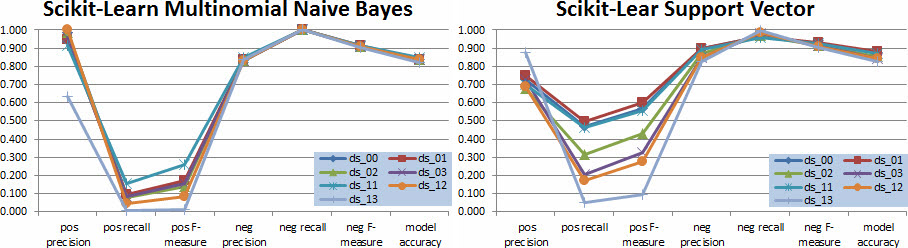
\includegraphics[width=1\textwidth]{Figures/Chapter5/scikit_process_chart_01.jpg}
	\caption[Scikit-Learn model performance using default parameters]{Graph showing the performance of the Scikit-Learn Multinomial Naive Bayes and Linear Support Vector learners using the default parameters}
	\label{fig:scikit_process_chart_01}
\end{figure}
 
It is immediately apparent that neither learner has performed well when predicting the positive class, but it is clear that the Naive Bayes classifier has performed particularly badly. Both models returned good results predicting the negative class with the Support Vector classifier performing the better of the two. However, with the use of Scikit-Learn it is also possible to dig deeper into these performances by analysing the confusion matrices for each of the datasets and models. Table \ref{tab:chapter5:nb_confusion_01} and Table \ref{tab:chapter5:sv_confusion_01} both give sample matrices, and it can be seen that the Naive Bayes model nearly exclusively predicted all samples as negative and although the Support Vector model managed to achieve better results it still favoured the negative class. The extreme examples are the performance of the models on dataset 13. In total, the Support Vector model only predicted 17 positive samples and the Naive Bayes model only predicted 3 positive samples or less than 1.5\% of the total possible number. It was assumed that the first simple NLTK models were also only predicting negative classes so Scikit-Learn providing this extra information is an advantage.

As five-fold cross validation was used this meant that five confusion matrices, one for each execution, were generated. It should be noted that the confusion matrices show in Tables \ref{tab:chapter5:nb_confusion_01} and Table \ref{tab:chapter5:sv_confusion_01} are actual numbers from one of the models and not averages as calculating averages would not make any sense.

\begin{table}[h]
	\centering
	\caption[Confusion matrices from the initial Scikit-Learn Naive Bayes model]{Table giving summary confusion matrix results for each test dataset from the initial Scikit-Learn Naive Bayes model}
	\label{tab:chapter5:nb_confusion_01}
	\begin{tabular}{lrrrrrrr}
		\toprule
		& \textbf{ds\_00}  & \textbf{ds\_01} & \textbf{ds\_02} & \textbf{ds\_03} & \textbf{ds\_11} & \textbf{ds\_12} & \textbf{ds\_13}   \\
		\midrule
		Pos Samples & 335 & 328 & 320 & 309 & 352 & 276 & 211 \\
		Neg Samples & 1580 & 1581 & 1466 & 1327 & 1536 & 1333 & 982 \\
		\midrule
		Pred Pos True Pos & 35 & 34 & 30 & 28 & 59 & 21 & 2 \\
		Pred Pos True Neg & 0 & 5 & 0 & 0 & 7 & 0 & 1 \\
		Pred Neg True Neg & 1580 & 1576 & 1466 & 1327 & 1529 & 1333 & 981 \\
		Pred Neg True Pos & 310 & 294 & 290 & 281 & 293 & 255 & 209 \\
		
		\bottomrule
    \end{tabular}
\end{table}

\begin{table}[h]
	\centering
	\caption[Confusion matrices from the initial Scikit Support Vector model]{Table giving summary confusion matrix results for each test dataset from the initial Scikit Support Vector model}
	\label{tab:chapter5:sv_confusion_01}
	\begin{tabular}{lrrrrrrr}
		\toprule
		& \textbf{ds\_00}  & \textbf{ds\_01} & \textbf{ds\_02} & \textbf{ds\_03} & \textbf{ds\_11} & \textbf{ds\_12} & \textbf{ds\_13}   \\
		\midrule
		Pos Samples & 353 & 335 & 306 & 295 & 361 & 292 & 212 \\
		Neg Samples & 1562 & 1574 & 1471 & 1341 & 1527 & 1317 & 981 \\
		\midrule
		Pred Pos True Pos & 172 & 173 & 104 & 64 & 163 & 61 & 12 \\
		Pred Pos True Neg & 67 & 49 & 66 & 22 & 56 & 19 & 5 \\
		Pred Neg True Neg & 1495 & 1525 & 1405 & 1319 & 1471 & 1298 & 976 \\
		Pred Neg True Pos & 181 & 162 & 202 & 231 & 198 & 231 & 200 \\
		
		\bottomrule
    \end{tabular}
\end{table}

A very interesting performance measure, that has only been briefly mentioned thus far, is the length of time each model takes to run. An examination of the run times for the first NLTK model and these first Scikit-Learn models showed that the Scikit-Learn models were between 87.5\% and 90.5\% faster with executions times around 1 second compared to 10 seconds for the NLTK models. This is a significant discovery. Given a choice between two models that have similar performance measurements, but one is ten times faster, the model chosen would always be the faster model. Hopefully this runtime advantage is maintained as more complexity is added to the Scikit-Learn models and the other performance measures are on a par with or better than the NLTK models. The time comparisons are shown in Figure \ref{fig:runtime_comp}.

\begin{figure}[htbp]
	\centering
	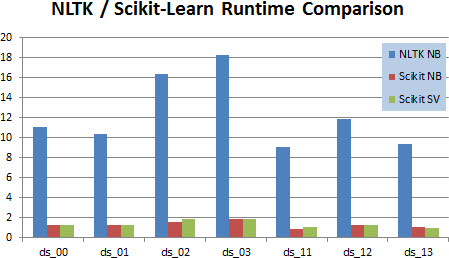
\includegraphics[width=.75\textwidth]{Figures/Chapter5/runtime_comp.jpg}
	\caption[NLTK - Scikit-Learn runtime comparison]{Graph showing the difference in runtime performance between the NLTK and Scikit-Learn}
	\label{fig:runtime_comp}
\end{figure}

\subsection{Further Exploration}
As with the NLTK model it is important to now examine some of the additional options offered by the Scikit-Learn TF-IDF implementation and also the Naive Bayes and Support Vector classifiers to determine if the model performance can be further improved before addressing the class imbalance. First the TF-IDF implementation will be examined.

The \verb|TfidfVectorizer| object performs two main tasks. The first is to convert a collection of text documents, in this case the array of training questions, into a matrix that is a sparse representation of token counts. It then transforms this count matrix into a term frequency inverse document frequency (TF-IDF) representation. In all, there are over twenty parameters that can be used to customise and fine tune the performance of this operator but for this research project only the following will be examined \cite{scikit-learn}:

\begin{enumerate}

	\item \textbf{ngram\_range}: tuple (min\_n, max\_n) \\
	The lower and upper boundary of the range of n-values for different n-grams to be extracted. All values of n such that $min_n <= n <= max_n$ are used.
	
	\item \textbf{stop\_words}: string {'english'}, list, or None (default) \\
	\verb|english| is currently the only supported string value and this has the affect of removing English stop words.
	
	\item \textbf{max\_df}: float in range [0.0, 1.0] or int, optional, 1.0 by default \\
	When building the vocabulary ignore terms that have a term frequency strictly higher than the given threshold.
	
	\item \textbf{norm}: 'l1', 'l2' or None, optional \\
	Norm used to normalize term vectors where \verb|l1| is the Manhattan Norm, $\lVert{x}\rVert = \sum_i \lvert x_i \rvert$, and \verb|l2| is the Euclidean Norm, $\lVert{x}\rVert = \sqrt{\sum_i \lvert x_i^2 \rvert}$. None is for no normalization.
	

\end{enumerate}

Other parameters allow preprocessing of the corpus, similar to that described in Chapter \ref{chapter4}, and more advanced control of the TF-IDF calculation, but these were not considered.

In total six models of interest were examined, all of which were based on \verb|dataset_01|, uni-grams without stop words removed. Three were based on the Naive Bayes classifier and three on the Support Vector classifier. The first model of each classifier type used the \verb|stop_words| parameter to remove frequently occurring tokens and these execution runs were called \verb|run_01| and \verb|run_04|. The second and third iteration of each model used the \verb|ngram_range| parameter to specify the use of bi-grams,\verb|run_02| and \verb|run_03|, and tri-grams \verb|run_05| and \verb|run_06|. What is different with the Scikit-Learn N-Gram parameter, when compared with the NLTK version, is that the Scikit-Learn retains all the n-grams in the range specified. For example, when \verb|ngram_range(1, 3)| is specified, this means that all uni-grams, bi-grams and tri-grams will be returned. The performance results from the execution of these six models is shown in Figure \ref{fig:scikit_process_chart_02}.

\begin{figure}[htbp]
	\centering
	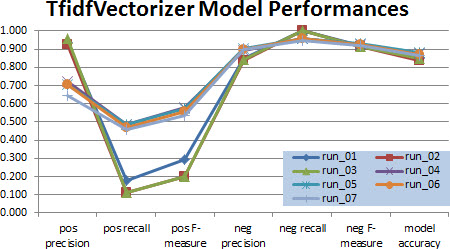
\includegraphics[width=.6\textwidth]{Figures/Chapter5/scikit_process_chart_02.jpg}
	\caption[Scikit-Learn model performance with default parameters]{Graph showing the performance of the Scikit-Learn Multinomial Naive Bayes and Linear Support Vector learners using the default parameters}
	\label{fig:scikit_process_chart_02}
\end{figure}

Comparing Figures \ref{fig:scikit_process_chart_01} and \ref{fig:scikit_process_chart_02}, and from an analysis of the details of the results, it is clear that there was an overall improvement in the models. Though this improvement was especially seen in the models that utilised bi-grams and tri-grams, models \verb|run_02, 03, 05 & 06|, the improvement was attributed to the inclusion of uni-grams. This fact was borne out by testing these models again without including uni-grams, \verb|ngram_range(2, 3)|. This yielded similarly disappointing performance results to the models utilising the original bi-grams and tri-grams only datasets. The inclusion or the \verb|norm| parameter did show a very slight improvement of less than 1\% in the performance of the models but the \verb|max_df| appeared to have little or no affect at all. The \verb|TfidfVectorizer| is now as shown in Listing \ref{lst:chapter5.3:snipet_04}.

\begin{lstlisting}[caption={TfidfVectorizer parameters}, label=lst:chapter5.3:snipet_04]
tfidf = TfidfVectorizer(
      stop_words='english'
    , ngram_range=(1, 3)
    , norm='l2'
)
\end{lstlisting}

Looking next at the Multinomial Naive Bayes classifier the only obvious parameter to consider at this stage is the \verb|alpha| parameter which is an additive Laplace smoothing parameter. Values of \verb|alpha| of 0.1, 0.01, 0.001 and 0.0001 were tested. Although all values returned improved results when compared with the default value of 1 it appeared that 0.001 gave slightly better results than the others. The performance measures returned when the value of \verb|alpha| was set to 0.001 is also shown in Figure \ref{fig:scikit_process_chart_02} as \verb|run_07|. It is clearly seen that introducing the \verb|alpha| parameter has significantly improved the predictive performance of the Naive Bayes classifier bringing its results in line with the Support Vector learner. Whilst there are Support Vector parameters that could be modified to possibly improve the performance of the model they are more associated with addressing class imbalance so they have been left to the next section where this topic is addressed.

It should be pointed out at this stage that the analysis of the parameters in this section is very much based on observation and manual analysis of the performance results returned. In the next section, a more scientific grid based approach will be used in order to fine tune the parameter values.

